\subsubsection{Comunicación interna $M_{23}$}

Por medio de estos enlaces internos, el sistema estará intercambiando información de forma constante entre los diferentes módulos con el fin de conocer el estado del proceso y tomar decisiones para realizar las operaciones para llevar a cabo las tareas del proceso de compostaje.

Existen 3 vías de comunicación (figura \ref{fg:convia}), la primera es una vía unidireccional, la cual será la encargada de enviar toda la información que se genera al interior del recipiente de compostaje, esta información contiene el valor de la temperatura y la humedad al interior del contenedor. Con esta información, la unidad de procesamiento será capaz de tomar decisiones sobre los actuadores.

Existe otra vía de comunicación unidireccional, la cual será la encargada de realizar las interacciones de con los actuadores del sistema (Sistema de riego, Sistema de ventilación, Sistema de temperatura y Sistema de aeración). Estas señales se encargan de la activación de los actuadores después del procesamiento de la información en el controlador. 

Por último, existe una vía de comunicación bidireccional, esta vía es la Interfaz Humano - Máquina, esta vía envía los datos que se generan al interior del proceso y a su vez, recibe algunas instrucciones desde el exterior. 

Para la implementación física de estos buses de comunicación, se planteó la conexión por medio de cables dupont, los cuales estarán conectados por medio de headers que se colocaran en las PCB que se estén desarrollando para los sistemas electrónicos del sistema.

\begin{figure}[h!]
            \centering
            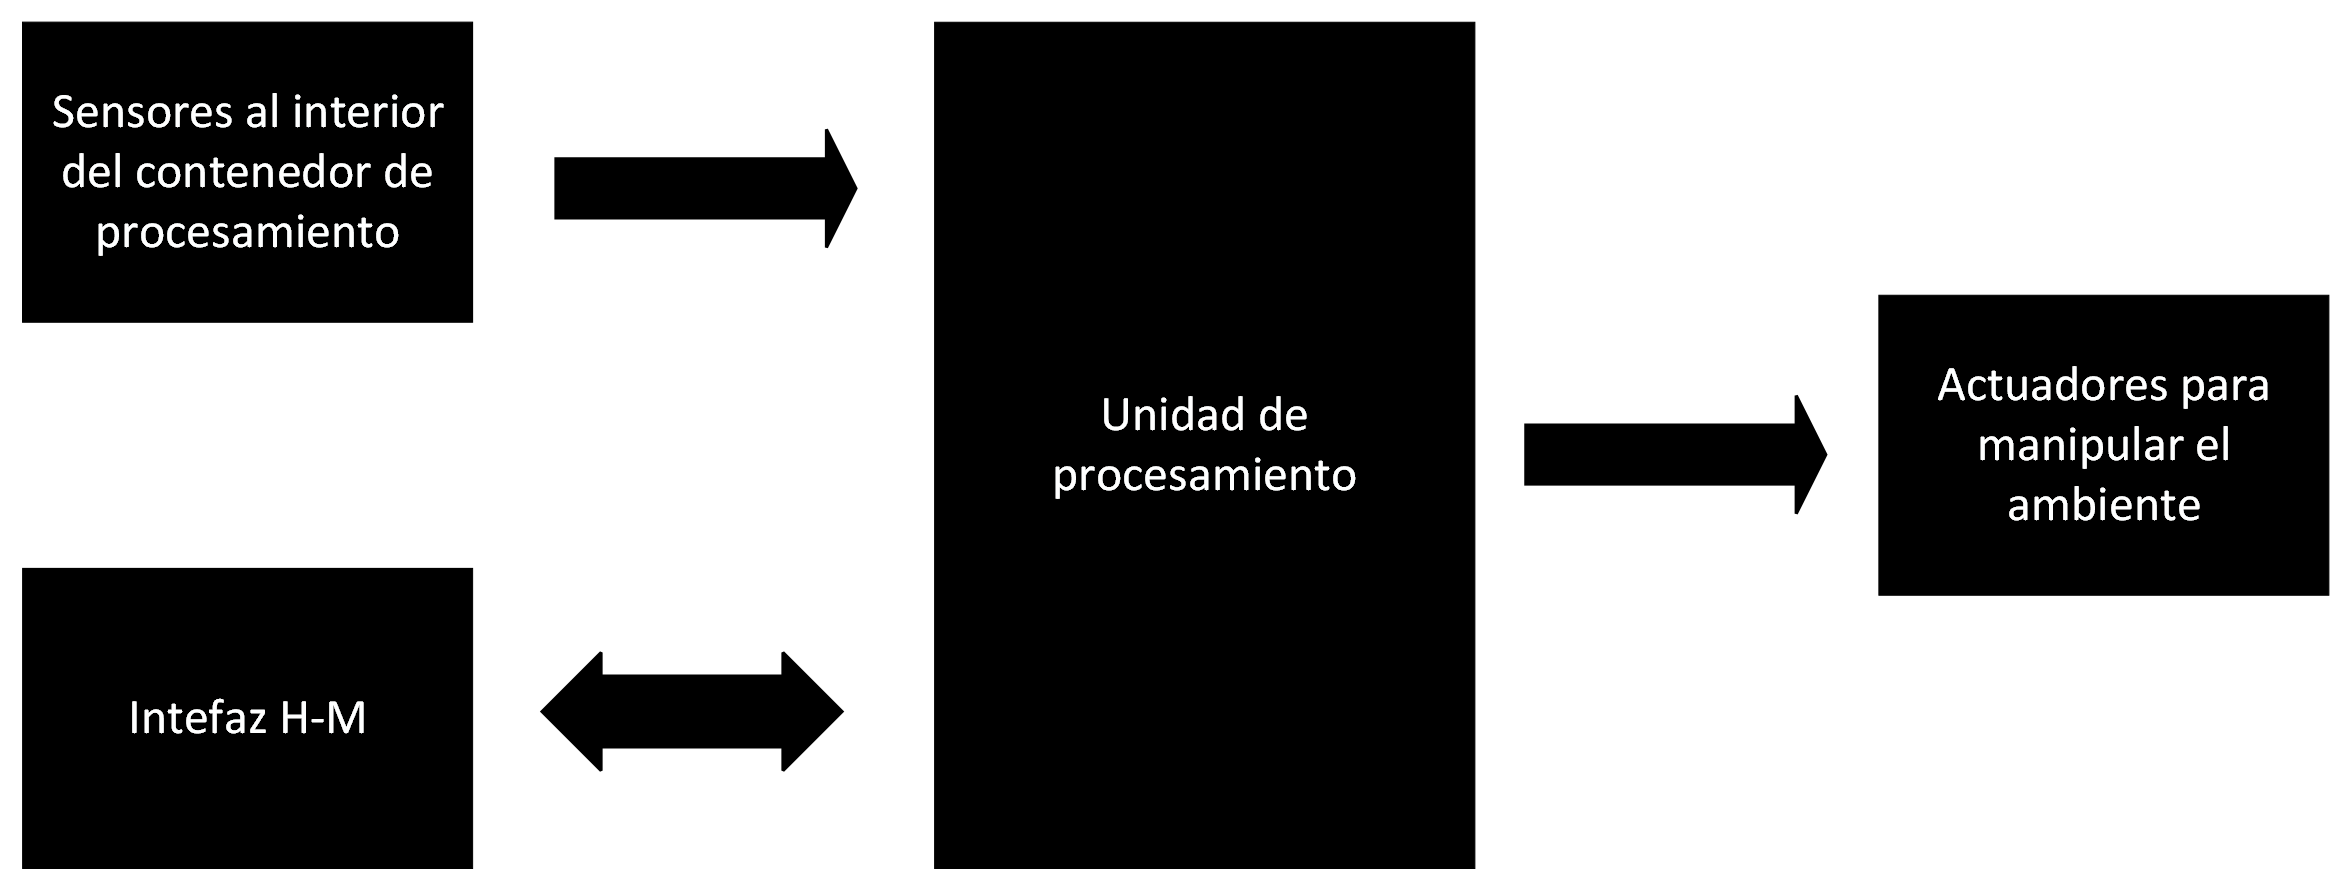
\includegraphics[scale=0.7]{images/Capitulo 4/Canales de comunicacion.png}
            \caption{Salidas y entradas de comunicación con la unidad de procesamiento}
            \label{fg:convia}
        \end{figure}